\documentclass[../../main]{subfiles}
\begin{document}

\label{ss:server-implementation-choices}
\subsection{Server implementation choices}
The server is that part that allow the user to manipulate his data and ask for recommendation under certain situation.
It also implement the security mechanism to avoid backtracking of the user while answering to recommendation request.
We decide to build the server in Nodejs after building a model in Python to adopt the use of different language and also
have the model and the APIs server on two different container. 

\begin{figure}[h]
    \centering
    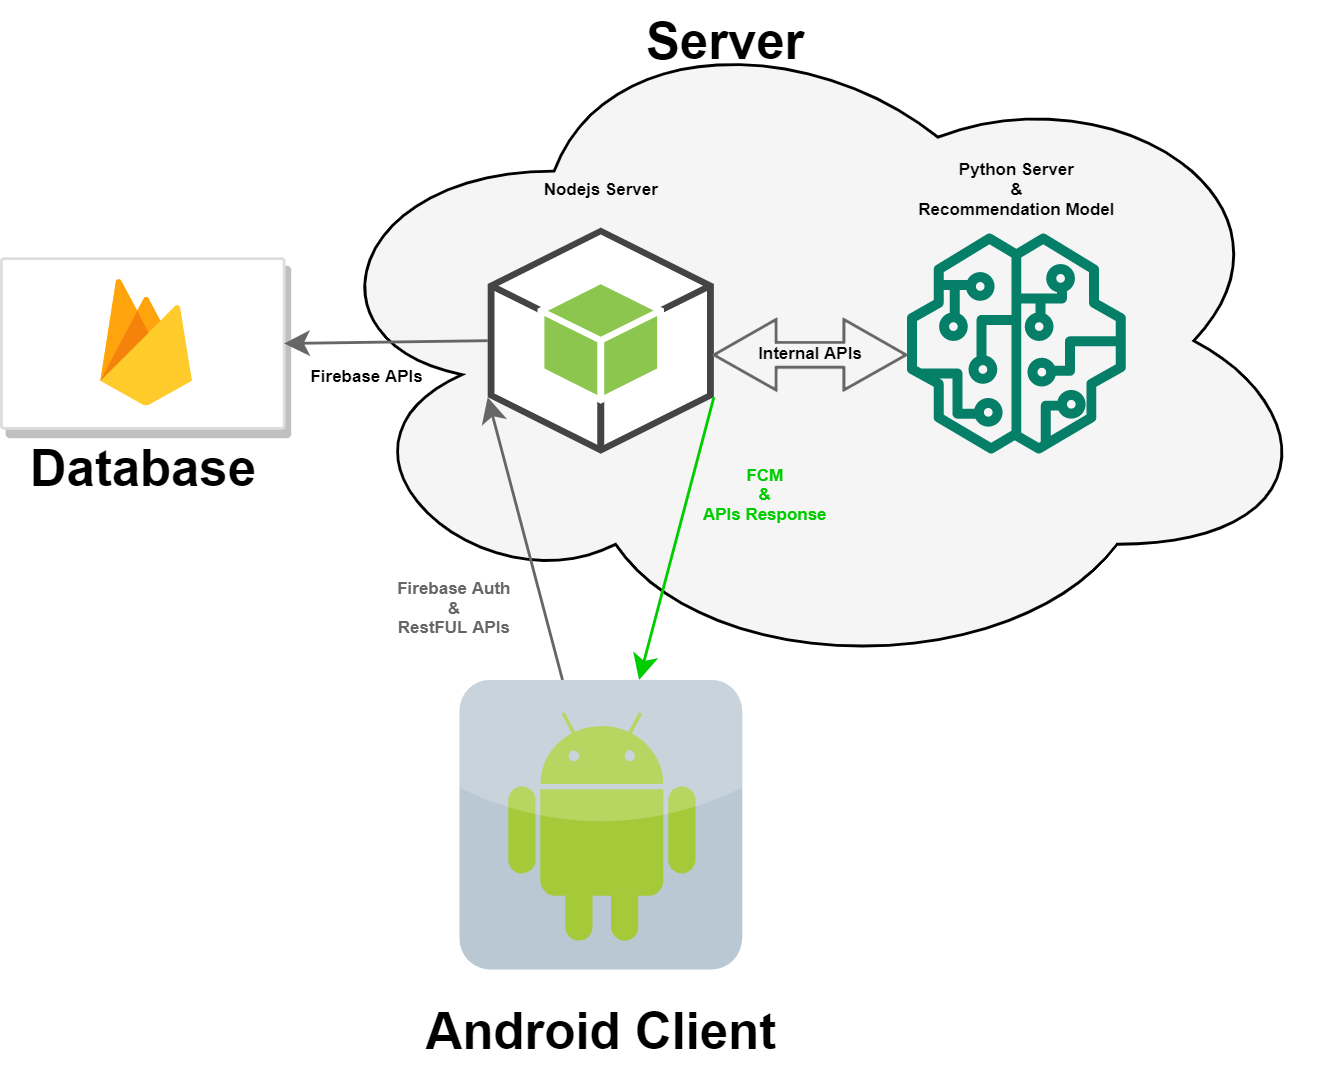
\includegraphics[width=0.8\textwidth]{images/system_architecture}
    \caption{Overall System Architecture}\label{fig:system_architecture}
\end{figure}

\subsubsection{Nodejs Server}
The Node server is used to handle the communication with:
\begin{itemize}
    \item Firestore Database, via Firebase APIs;
    \item Android Client, via RESTful APIs and FCM;
    \item Python Server, via Internal RESTful APIs;
\end{itemize}

\paragraph{RESTful APIs}
The clients and the Nodejs server communicate via RESTful APIs, but the server can also send FCM message, received as push notification, to the client.
The recommendation api were made as POST also if they don't actually post any data until the \textbf{/recommendation/train} but for semplicity we build
them like this so we can encrypt the message of the body instead of query string.
The APIs are divided into three main category that respectively allow the user to:
\begin{itemize}
    \item Authentication: authenticate, save notification token and his public key;
    \item Database: manipulate and retrieve data;
    \item Recommendation: receive a recommendation and retrain model with feedback.
\end{itemize}

%\item 
\begin{enumerate}[I)]
    \item \textbf{Authentication}:
    \begin{itemize}
        \item \textbf{'/user-data'}
        \begin{enumerate}[i)]
            \item \textbf{'/notification-token'} Save notification token (POST);
            \item \textbf{'/public-key'} Save user RSA public key (POST);
        \end{enumerate}
    \end{itemize}
    
    \item \textbf{Database}:
    \begin{itemize}
        \item Points of Interest \textbf{'/points-of-interest'}:
        
        \begin{enumerate}[i)]
            \item \textbf{'/'} Get pois list (GET);
            \item \textbf{'/add'} Add a poi (POST);
            \item \textbf{'/remove'} Remove a poi (DELETE);
        \end{enumerate}
    
        \item Live Events \textbf{'/live-events'}:
        \begin{enumerate}[i)]
            \item \textbf{'/'} Get live events list (GET);
            \item \textbf{'/add'} Add a live event (POST);
        \end{enumerate}
    
        \item Friends \textbf{'/friends'}:
        \begin{enumerate}[i)]
            \item \textbf{'/'} Get friends list (GET);
            \item \textbf{'/add'} Add a friend request (POST);
            \item \textbf{'/confirm'} Confirm a friend request (POST);
            \item \textbf{'/deny'} Deny a friend request (POST);
            \item \textbf{'/remove'} Remove a friend (DELETE);
        \end{enumerate}
    \end{itemize}
    \item \textbf{Recommendation}:
    \begin{itemize}
        \item \textbf{'/recommendation'}
        \begin{enumerate}[i)]
            \item \textbf{'/places'} Get a place recommendation (POST);
            \item \textbf{'/validity'} Get validity for a specific place (POST);
            \item \textbf{'/train'} Train model with user's feedback (POST)
        \end{enumerate}
    \end{itemize}
\end{enumerate}
    

    
\subsubsection{Recommendation Model}
After the data synthetization we build the dataset used as input to train our model. First of all we separeted the place cateogry columns because it represent the results that we want to predict, and we removed some useless information from the dataset like the data returned from Places API and the cluster index.
\paragraph*{Oversample}
We oversampled the dataset with two mechanism:
\begin{itemize}
    \item \textbf{RandomOverSampler} from imblearn;
    \item \textbf{get\_dummies} from pandas.
\end{itemize}

We used RandomOverSampler to oversample X and y, and get\_dummies to oversample X relative to human activity
because they are saved as string. We also one hot encoding the human activity to give more meaning to this value on the dataset.

\paragraph*{Train}
We used the 70\% of the dataset to perform the training and we used a \textbf{Decision Tree Classifier} to train a model able to
predict the place category. 
With a request input made of:
\begin{itemize}
    \item Seconds of day;
    \item Day of week;
    \item Latitude;
    \item Longitude;
    \item Human activity encoded.
\end{itemize}
As said in \namerefLabeled{paragraph:train_design} we thought that the recommendation model should follow a path like \textit{' At this \textbf{Hour} in this \textbf{Day} in this \textbf{position} by doing this \textbf{human activity} the best place is \textbf{place category}. '}.
Talking about node of the tree. This is due the fact we want to discriminate determinate category by the time of the day and the human activity we are performing.
Ideally a user goes to the gym during the week but probably in the evening or early morning, 
goes to a restaurant/bar in any day at breakfast, launch or dinner time and he is probably walking or still on that place.
But probably he goes to some leisure place during the weekend in the middle morning, afternoon or any day after dinner in the evening/night.

The latitude and longitude is used to further discriminate some activity in any places because the data collected from the users could change due to their different attitude in the various part of the world.
(Most of the point are from USA or China)
\paragraph*{Test}
After the train we tested the model obtained with the remaining 30\% of the oversampled dataset and we have instantly obtained and accuracy neart to 65\%, that is very high due to the small dataset that we obtained from the preprocessing.
Also we tried some recommendation request from the android client emulator and we received decent predictions. To continue improving the model we implemented the possibility to retrain it by adding the recommendation that the client has received, modified with the right category if he feels that the prediction didn't suit his needs. 

\subsubsection{Security}
Obviously we had to implement some security mechanism to avoid tracking of the user.\\ We decided to generate an HTTPS certificate for the server and 
a pair of public/private key for both server and client to allow an RSA encrypted communication.
\paragraph{HTTPS}
\noindent{First of all we generate an https certificate for the nodejs server with \textbf{openssl} by doing:\newline}
\begin{lstlisting}[language=bash]
$ openssl req -x509 -newkey rsa:4096 -keyout https_private.pem 
-out https_public.pem -sha256 -days 365
\end{lstlisting}
And a public key in bks for the client android so it can trust our server.
\paragraph*{RSA Encryption}
The data about poi, live events and friends is sent and saved in plain on the database, since they can add any of those from everywhere they don't represent sensitive data about the user.
But the recommendation are based on the actual position and this need to be obfuscated.
\\Firstly we have thinked about using cloacking but this could be bad for the prediction doing to the possibility of multiple poi near the user.
\\After that we thought also to use Dummy updates but to retrain model with the feedback of the user we need to send the actual position and the server doesn't know it because only the client knows.
\\So we decided to implement a \textbf{Location Privacy Protection Mechanism} by using as function, to obscure the sensitive information, RSA encryption.
\\This seems to suit our case because we need to exchange only the public key that is useless to decrypt the message, and even if it is sniffed and someone try to send a request to our server he still needs the firebase token from firebase auth.
\noindent We generate the keys in this way:
\begin{lstlisting}[language=bash]
$ openssl genrsa -out recommendation_private_key.pem 4096
$ openssl rsa -in recommendation_private_key.pem -pubout 
    -outform PEM -out recommendation_public_key.pem 
$ openssl rsa -in recommendation_private_key.pem -pubout 
    -outform DER -out server_key.der
\end{lstlisting}
The first command generate a 4096 bytes long private key for the server, the second one his public key and the last one generate a public key in \.der extension for the android client so it can encrypt message for the server.
We generate the pair of keys in the client once, directly from the phone by using andriod KeyStore Library, and save them in the android keystore directory.

\end{document}